\documentclass[10pt]{beamer}

%%%
% PREAMBLE FOR THIS DOC 
%%%
%https://tex.stackexchange.com/questions/68821/is-it-possible-to-create-a-latex-preamble-header
\usepackage{/Users/miw267/Repos/csci246_fall2025/slides/preambles/beamer_preamble_for_CSCI246}


%%%
% PREAMBLE SPECIAL FOR THIS DECK
%%%
\definecolor{condred}{RGB}{200,30,30}
\definecolor{accessgreen}{RGB}{30,160,60}
\usetikzlibrary{calc}


%%% TRY TO RESHOW TOC AT EACH SECTION START (with current section highlighted)
% Reference: https://tex.stackexchange.com/questions/280436/how-to-highlight-a-specific-section-in-beamer-toc
\newcommand\tocforsect[2]{%
  \begingroup
  \edef\safesection{\thesection}
  \setcounter{section}{#1}
  \tableofcontents[#2,currentsection]
  \setcounter{section}{\safesection}
  \endgroup
}


%%%% HERES HOW TO DO IT CORRECTLY
% FIRST IN .STY FILE, DO
%\usetheme[sectionpage=none]{metropolis}
% THEN AT EACH SECTION DO
%\begin{frame}{Outline}
%  \tableofcontents[currentsection]	
%\end{frame}



%\setbeamertemplate{navigation symbols}{}
%\setbeamertemplate{footline}[frame number]{}


%%%
% DOCUMENT
%%%

\begin{document}

%\maketitle

%% Title page frame
%\begin{frame}
%    \titlepage 
%\end{frame}





\title{09/05/2025: Multiple Proofs}
\author{CSCI 246: Discrete Structures}
\date{Textbook reference: Ch. 2, Hampkins}

\begin{frame}
    \titlepage 
\end{frame}


\begin{frame}


\begin{mygreenbox}[title=Quiz Set up]
\begin{itemize}
\item \textbf{Guest lecturer Monday}: Paul Cornish.   
\end{itemize}
\end{mygreenbox}

\vfill 

\begin{myyellowbox}[title=Today's Agenda]
\begin{itemize}
	\item Weekly quiz (20 mins)
	\item Review ($\approx$ 10 mins)
	\item Group exercises  ($\approx$ 10 mins)
	\item Review group exercises ($\approx$ 10 mins)
\end{itemize}

\end{myyellowbox}



\end{frame}






\begin{frame}
\small 
 \begin{myredbox}[title=Weekly Quiz] 
\begin{enumerate}
	\item  \textit{(Sec. 6 -- Counterexample.)}  Disprove the following conjecture: \textit{Let $a$ and $b$ be integers.  If $a|b$ and $b|a$, then $a=b$.}
	\item \textit{(Sec. 7 -- Boolean Algebra.)} DeMorgan's laws are:
	\[ \lnot (x \land y) = (\lnot x) \lor (\lnot y) \quad \text{and} \quad \lnot (x \lor y) = (\lnot x) \land (\lnot y) \]
	Prove the first of these (using truth tables). 
	\item \textit{(Sec. 7 -- Boolean Algebra.)}  Use DeMorgan's law to show how to disprove an if-and-only-if statement.
\end{enumerate}
\end{myredbox}

\vfill 
\begin{mygreenbox}[title=Reference Material: Scheinerman Definition 3.2] Let $a$ and $b$ be integers.  We say $a$ is \textit{divisible} by $b$, written $b \mid a$, provided there is an integer $c$ such that $bc=a$. 	
\end{mygreenbox}

\vfill 
\begin{myyellowbox}[title=Notation reminder]
\[
\begin{array}{rclcrclcrcl}
\lnot & : & \texttt{not} &\qquad \qquad & \lor     & : & \texttt{or}    \qquad \qquad &  & \land & : & \texttt{and}
\end{array}
\]
\end{myyellowbox}

\end{frame}



\begin{frame}{Intermezzo: Why are we doing all of this?}


\colorbox{red!30}{\textbf{Objection.}} Why should computer scientists be concerned with formal structures (definitions, theorems, logic, etc.)?

\pause 
\vfill \vfill 
\colorbox{green!30}{\textbf{Example: Application of \qq{Iff} to Cybsercurity.}} In security, \qq{iff} statements are important because a one-way implication (\qq{if}) is not enough.
\pause 
For example,
\begin{itemize}
	\item \textit{If a password is correct, then access is granted.} (Ok, but what if access is sometimes granted without a password?) \pause 
	\item  The iff ensures no unintended backdoors or bypasses. \pause 
\end{itemize}


In general, the iff condition captures both \textbf{soundness} (no false accepts) and \textbf{completeness} (no false rejects).
\end{frame}

\begin{frame}{Soundness and Completeness of an Authentication System (Venn examples)}

\centering
\begin{tabular}{cc}
% 1: neither sound nor complete
\begin{minipage}{0.45\linewidth}\centering
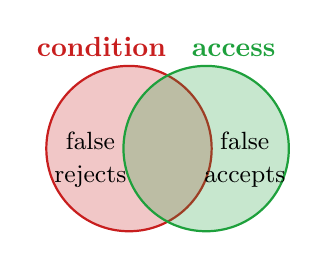
\begin{tikzpicture}[scale=0.7]
  \def\r{1.5}
  \coordinate (C1) at (-0.7,0);
  \coordinate (A1) at ( 0.7,0);
  \draw[fill=condred, fill opacity=0.25, draw=condred, thick] (C1) circle (\r);
  \draw[fill=accessgreen, fill opacity=0.25, draw=accessgreen, thick] (A1) circle (\r);
  \node[condred,above] at ($(C1)+(-0.5,1.5)$) {\textbf{condition}};
  \node[accessgreen,above] at ($(A1)+(0.5,1.5)$) {\textbf{access}};
  \node[align=center] at ($ (C1) + (-0.7,-0.2) $) {\small false\\ \small rejects};
  \node[align=center] at ($ (A1) + (0.7,-0.2) $) {\small false\\ \small accepts};
\end{tikzpicture}

\small\textbf{neither sound nor complete}
\end{minipage}
&
% 2: sound but not complete
\begin{minipage}{0.45\linewidth}\centering
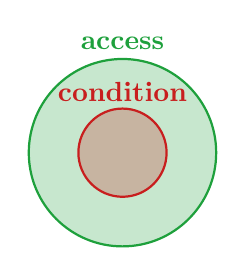
\begin{tikzpicture}[scale=0.7]
  \draw[fill=accessgreen, fill opacity=0.25, draw=accessgreen, thick] (0,0) circle (1.7);
  \draw[fill=condred, fill opacity=0.25, draw=condred, thick] (0,0) circle (0.8);
  \node[condred,above] at (0,0.75) {\textbf{condition}};
  \node[accessgreen,above] at (0,1.7) {\textbf{access}};
\end{tikzpicture}

\small\textbf{complete (no false rejects) but not sound}

\end{minipage}
\\[1em]

% 3: complete but not sound
\begin{minipage}{0.45\linewidth}\centering
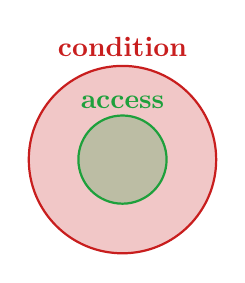
\begin{tikzpicture}[scale=0.7]
  \draw[fill=condred, fill opacity=0.25, draw=condred, thick] (0,0) circle (1.7);
  \draw[fill=accessgreen, fill opacity=0.25, draw=accessgreen, thick] (0,0) circle (0.8);
  \node[condred,above] at (0,1.7) {\textbf{condition}};
  \node[accessgreen,above] at (0,0.75) {\textbf{access}};
\end{tikzpicture}

\small\textbf{sound (no false accepts) but not complete}
\end{minipage}
&
% 4: sound and complete
\begin{minipage}{0.45\linewidth}\centering
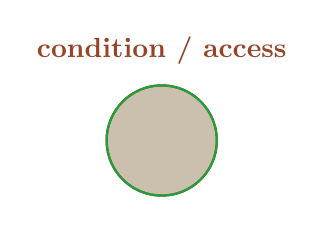
\begin{tikzpicture}[scale=0.7]
  \draw[fill=condred, fill opacity=0.25, draw=condred, thick] (0,0) circle (1.0);
  \draw[fill=accessgreen, fill opacity=0.18, draw=accessgreen, thick] (0,0) circle (1.0);
  \node[condred!70!accessgreen,above] at (0,1.2) {\textbf{condition / access}};
\end{tikzpicture}

\small\textbf{sound and complete}
\end{minipage}
\end{tabular}

\end{frame}


\begin{frame}[standout]

Review additional group exercises \\
from Boolean Algebra 
	
\end{frame}



%
%\begin{frame}{Multiple Proofs}
%
%\begin{mygreenbox}[title=Quote of the Day]
%“Perhaps the greatest pleasure of mathematics is that, as you try to solve problems, you find that you come to understand new techniques. You see the problem \textbf{from a different perspective}, and that’s when you make progress.”  \\
%
%-- Andrew Wiles (who famously solved Fermat's Last Theorem)
%\end{mygreenbox}
%	
%\vfill \vfill 
%\begin{myredbox}[title=Role of this chapter]
%\begin{itemize}
%\item To demonstrate \textit{perspective shifting} in mathematics: its existence, beauty, and value.
%\item Another chance to practice theorems and proofs.	
%\end{itemize}
%
%	
%\end{myredbox}
%
%\end{frame}




%
%\begin{frame}{Resolving a puzzle from earlier}
%\footnotesize 
%\begin{myyellowbox}[title=Puzzle]
%In Sec. 5 (Proofs), we showed that  \textit{zero is divisible by zero} ($0|0$). How can we make sense of this? Many of us have been told that we ``can't divide by 0". \end{myyellowbox}
%\pause 
%\vfill 
%	\begin{mydef}[title=Reminder of Definition 3.2 (\textbf{Divisible})]
%	Let $a$ and $b$ be integers.  We say that $a$ is \textit{divisible} by $b$ provided there is an integer $c$ such that $bc=a$. The notation for this is $b|a$. 
%	\end{mydef}
%\vfill 
%\begin{myredbox}[title=Observations]   
%\begin{itemize}
%\item  Although $\frac{b}{a}$ is a \textbf{number},  the above shows that $b|a$ is a \textbf{proposition}. 
%\item 	We don’t have $0|1$ (\texttt{False}), but we do have $0|0$ (\texttt{True}).   
%\end{itemize}
%\end{myredbox}
%
%\begin{myyellowbox}[title=Resolution to Puzzle]
%\begin{itemize}
%\item $\frac{x}{0}$ is problematic, since not all $x$ are divisible by 0.   ($0|x$ is \texttt{False} for all integers $x$ except $x=0$.)
%\item If we take $x=0$, we do have $0|0$, but we don't know what number  $\frac{0}{0}$ equals (i.e. $c$ in the definition could be any integer).  %[In calc, this is an \text{indeterminate form}.]
%\end{itemize}
%
%\end{myyellowbox}
%
%%In calculus, \#1 is considered infinity, and \#2 is considered an indeterminate form.
%
%\end{frame}


\begin{frame}{Group work}


\begin{myyellowbox}[title=Announcements about group work]
\begin{itemize}
	\item Ideas if you get stuck during group exercises:
	\begin{itemize}
	\item[(a)] Get my/Paul's attention. 
	\item[(b)] Find other group to give a hint/lead.
	\item[(c)] Use textbook as resource.
	\end{itemize} 
	\item It's okay to get stuck! That's a \underline{natural} part of learning!
\end{itemize}	
\end{myyellowbox}
\vfill 
\begin{mygreenbox}[title=Quote of the Semester]
“The best way to learn is to do; the worst way to teach is to talk.” \\

-- Paul Halmos, a renowned mathematician and expositor
\end{mygreenbox}

\end{frame}




\begin{frame}{Random group assignments}
\footnotesize
\begin{columns}
\begin{column}{0.33\textwidth}
Aaron Christensen: 18 \\ 
Aidan Sinclair: 6 \\ 
Bennett Dijkstra: 15 \\ 
Brendan Kelly: 4 \\ 
Buggy Garza: 12 \\ 
Cedric Jefferson: 14 \\ 
Conner Brost: 2 \\ 
Connor Graville: 7 \\ 
David Knauert: 11 \\ 
David Oswald: 10 \\ 
Elias Martin: 4 \\ 
Ericson O'Guinn: 6 \\ 
Erik Halverson: 4 \\ 
Francis Bush: 14 \\ 
Garrett Miller: 3 \\ 
George Cutler: 10 \\ 
Georgia Franks: 13 \\ 
Gregor Schmidt: 5 \\\end{column}
\begin{column}{0.33\textwidth}
Hakyla Riggs: 15 \\ 
Izayah Abayomi: 6 \\ 
Jacob Ketola: 17 \\ 
Jacob Ruiz: 9 \\ 
Jaden Hampton: 9 \\ 
Jeremy Ness: 2 \\ 
Jonah Day: 8 \\ 
Karter Gress: 1 \\ 
Kyle Hoerner: 5 \\ 
Landry Clarke: 17 \\ 
Leon BirdHat: 13 \\ 
Lillian Ziegler: 2 \\ 
Matthew Rau: 16 \\ 
Matyas Kari: 3 \\ 
Micah Miller: 12 \\ 
Michael Pitman: 7 \\\end{column}
\begin{column}{0.33\textwidth}
Nathan Campbell: 7 \\ 
Nathan Hooley: 10 \\ 
Nicholas Rugani: 1 \\ 
Noah Andersson: 8 \\ 
Olivia Greuter: 13 \\ 
Peter Van Vleet: 16 \\ 
Pierce Dotson: 9 \\ 
Quinn Carlson: 5 \\ 
Ridley Christoferson: 15 \\ 
Riley Smith: 12 \\ 
Sierra Holleman: 1 \\ 
Tanner Gramps: 16 \\ 
Timothy True: 11 \\ 
Titus Sykes: 14 \\ 
Trey Randall: 3 \\ 
William Grant: 11 \\ 
William Sheldon: 8 \\ 
Zachary Reller: 17 \\\end{column}
\end{columns}
\end{frame}

\begin{frame}{Group exercises}

\begin{enumerate}
\item (Hamkins Ex. 2.1, first part) Prove that the sum, difference, and product of two even numbers is even.
\item (Hamkins Ex. 2.1, second part) Prove that the sum and difference of two odd numbers is even, but the product of two odd numbers is odd.
\end{enumerate}
\end{frame}



%
\begin{frame}{Solution to group exercise \#1}

\footnotesize 

\textbf{Proposition.} The sum, difference, and product of two even numbers is even.
\vfill 
\textbf{Proof.}
\begin{tabularx}{\textwidth}{|L{3.5cm}|X|}
\hline \textbf{Annotation} & \textbf{Main Text} \\ \hline
 \hlorange{Convert Prop. to ``if-then" form} &  \hlorange{We show that if $x$ and $y$ are even integers, then $x+y$, $x-y$, and $xy$ are even.} \\ \hline
\hlblue{State assumption (\qq{if})} & \hlblue{Let $x$ and $y$ be even integers} \\ \hline
\hlgreen{Unravel defs.} & \hlgreen{What goes here!?} \\ \hline
\hlred{*** The glue ***} &  \\
\hline
\hlgreen{Unravel defs.} & \hlgreen{What goes here!?} \\ 
\hline
  \hlblue{State conclusion (\qq{then})} & \hlblue{Hence, $x+y, x-y$ and $xy$ are even.} \\ \hline
\hline
\end{tabularx}
\end{frame}
%
%

%
\begin{frame}{Solution to group exercise \#1}

\footnotesize 

\textbf{Proposition.} The sum, difference, and product of two even numbers is even.
\vfill 
\textbf{Proof.}
\begin{tabularx}{\textwidth}{|L{3.5cm}|X|}
\hline \textbf{Annotation} & \textbf{Main Text} \\ \hline
 \hlorange{Convert Prop. to ``if-then" form} &  \hlorange{We show that if $x$ and $y$ are even integers, then $x+y$, $x-y$, and $xy$ are even.} \\ \hline
\hlblue{State assumption (\qq{if})} & \hlblue{Let $x$ and $y$ be even integers} \\ \hline
\hlgreen{Unravel defs.} & \hlgreen{Then by the definition of even, there exist integers $a,b$ such that $x=2a$ and $y=2b$.} \\ \hline
\hlred{*** The glue ***} & \hlred{What goes here?!?!} \\
\hline
 \hlgreen{Unravel defs.} & \hlgreen{So there are integers $c,d,e$ such that $x+y=2c$, $x-y=2d$, and $xy=2e$.} \\ \hline
  \hlblue{State conclusion (\qq{then})} & \hlblue{Hence, $x+y, x-y$ and $xy$ are even.} \\ \hline
\hline
\end{tabularx}
\end{frame}
%
%

\begin{frame}{Solution to group exercise \#1}
\footnotesize 
\textbf{Proposition.} The sum, difference, and product of two even numbers is even.
\vfill 
\textbf{Proof.}

\begin{tabularx}{\textwidth}{|L{3.5cm}|X|}
\hline \textbf{Annotation} & \textbf{Main Text} \\ \hline
\hlorange{Convert Prop. to \qq{if-then} form} &  \hlorange{We show that if $x$ and $y$ are even integers, then $x+y$, $x-y$, and $xy$ are even.} \\ \hline
\hlblue{State assumption (\qq{if})} & \hlblue{Let $x$ and $y$ be even integers} \\ \hline
\hlgreen{Unravel defs.} & \hlgreen{Then by the definition of even, there exist integers $a,b$ such that $x=2a$ and $y=2b$.} \\ \hline
\hlred{*** The glue ***} & 
\hlred{We have:
\[
\begin{aligned}
x+y &= 2a + 2b = 2\explaintermbrace{$\defeq c$}{(a+b)} \\	
x-y &= 2a - 2b = 2\explaintermbrace{$\defeq d$}{(a-b)} \\
xy  &= 2a \cdot 2b = 2\explaintermbrace{$\defeq e$}{(2ab)}  
\end{aligned}
\]
}
\\ \hline
 \hlgreen{Unravel defs.} & \hlgreen{So there are integers $c,d,e$ such that $x+y=2c$, $x-y=2d$, and $xy=2e$.} \\ \hline
  \hlblue{State conclusion (\qq{then})} & \hlblue{Hence, $x+y, x-y$ and $xy$ are even.} \\ \hline
\hline
\end{tabularx}
\end{frame}


\begin{frame}{Solution to group exercise \#2}
\footnotesize 
\textbf{Proposition.} The sum and difference of two odd numbers is even, but the product of odd numbers is odd.
\vfill 
\textbf{Proof.}

\begin{tabularx}{\textwidth}{|L{3.5cm}|X|}
\hline \textbf{Annotation} & \textbf{Main Text} \\ \hline
 \hlorange{Convert Prop. to ``if-then"} &  \hlorange{We show that if $x$ and $y$ are odd integers, then $x+y$ and $x-y$ are even, but $xy$ is odd.} \\ \hline
\hlblue{State ``if"} & \hlblue{Let $x$ and $y$ be odd integers.} \\ \hline
\hlgreen{Unravel defs.} & \hlgreen{What goes here?!?!} \\ \hline
\hlred{*** The glue ***} &  \\ \hline
\\ \hline
 \hlgreen{Unravel defs.} & \hlgreen{What goes here?!?!} \\ \hline
  \hlblue{State ``then"} & \hlblue{Hence,  $x+y$ and $x-y$ are even, but $xy$ is odd.} \\ \hline
\hline
\end{tabularx}
\end{frame}



\begin{frame}{Solution to group exercise \#2}
\footnotesize 
\textbf{Proposition.} The sum and difference of two odd numbers is even, but the product of odd numbers is odd.
\vfill 
\textbf{Proof.}

\begin{tabularx}{\textwidth}{|L{3.5cm}|X|}
\hline \textbf{Annotation} & \textbf{Main Text} \\ \hline
 \hlorange{Convert Prop. to ``if-then"} &  \hlorange{We show that if $x$ and $y$ are odd integers, then $x+y$ and $x-y$ are even, but $xy$ is odd.} \\ \hline
\hlblue{State ``if"} & \hlblue{Let $x$ and $y$ be odd integers.} \\ \hline
\hlgreen{Unravel defs.} & \hlgreen{Then by the definition of odd, there exist integers $a,b$ such that $x=2a+1$ and $y=2b+1$.} \\ \hline
\hlred{*** The glue ***} & \hlred{What goes here?!?!} \\ \hline
\\ \hline
 \hlgreen{Unravel defs.} & \hlgreen{So there are integers $c,d,e$ such that $x+y=2c$, $x-y=2d$, and $xy=2e+1$.} \\ \hline
  \hlblue{State ``then"} & \hlblue{Hence,  $x+y$ and $x-y$ are even, but $xy$ is odd.} \\ \hline
\hline
\end{tabularx}
\end{frame}




\begin{frame}{Solution to group exercise \#2}
\footnotesize 
\textbf{Proposition.} The sum and difference of two odd numbers is even, but the product of odd numbers is odd.
\vfill 
\textbf{Proof.}

\begin{tabularx}{\textwidth}{|L{2cm}|X|}
\hline \textbf{Annotation} & \textbf{Main Text} \\ \hline
 \hlorange{Convert Prop. to ``if-then"} &  \hlorange{We show that if $x$ and $y$ are odd integers, then $x+y$ and $x-y$ are even, but $xy$ is odd.} \\ \hline
\hlblue{State ``if"} & \hlblue{Let $x$ and $y$ be odd integers.} \\ \hline
\hlgreen{Unravel defs.} & \hlgreen{Then by the definition of odd, there exist integers $a,b$ such that $x=2a+1$ and $y=2b+1$.} \\ \hline
\hlred{* The glue *} & 
\scriptsize
\hlred{We have:
\[
\begin{aligned}
x+y &= (2a+1) + (2b+1) = 2a+2b+2 = 2\explaintermbrace{$\defeq c$}{(a+b+1)} \\	
x-y &= (2a+1) - (2b+1) = 2a - 2b = 2\explaintermbrace{$\defeq d$}{(a-b)} \\
xy &= (2a+1)\, (2b+1) = 4ab + 2a + 2b + 1 =2\explaintermbrace{$\defeq e$}{(2ab + a + b)} \, +1  	
\end{aligned}
\]}
\\ \hline
 \hlgreen{Unravel defs.} & \hlgreen{So there are integers $c,d,e$ such that $x+y=2c$, $x-y=2d$, and $xy=2e+1$.} \\ \hline
  \hlblue{State ``then"} & \hlblue{Hence,  $x+y$ and $x-y$ are even, but $xy$ is odd.} \\ \hline
\hline
\end{tabularx}
\end{frame}


\end{document}
